\section{Segmentation}

Segmentation is the process of dividing an image into distinct regions that should represent the objects in the image. For example in an application that monitors traffic congestion on a road, it would be useful count the number of cars in a video frame. To do this it’s important to distinguish between groups of pixels that belong to the background and those that belong to cars.

This application concerns itself with distinguishing between pixels that belong to healthy skin surrounding a lesion, and those that belong to the lesion itself.

\subsection{Thresholding}

Thresholding describes a family of segmentation techniques that group neighbouring pixels together based on the similarity of their intensity. Basically the image is converted to a greyscale image and pixels grouped based on whether their are above or below a ratio, and if they are adjoining.

The following figures \ref{fig:thresh_A} to \ref{fig:thresh_D} are examples of segmentation using thresholding with threshold values at 39\% and 50\%. The regions are grouped together based on adjacency and colour coded. Before thresholding, the images were equalised using CLAHE.

\begin{figure}[H]
    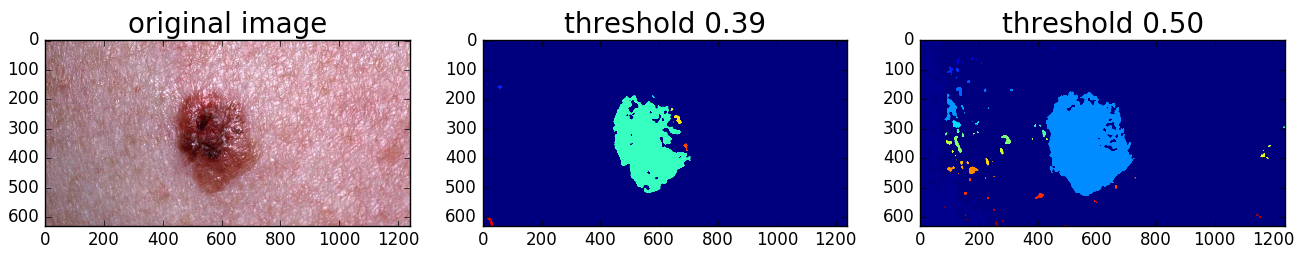
\includegraphics[width=\textwidth,keepaspectratio]{assets/image_processing/thresholding/figure_01.png}
    \caption{Threshold segmentation A}
    \label{fig:thresh_A}
\end{figure}
\begin{figure}[H]
    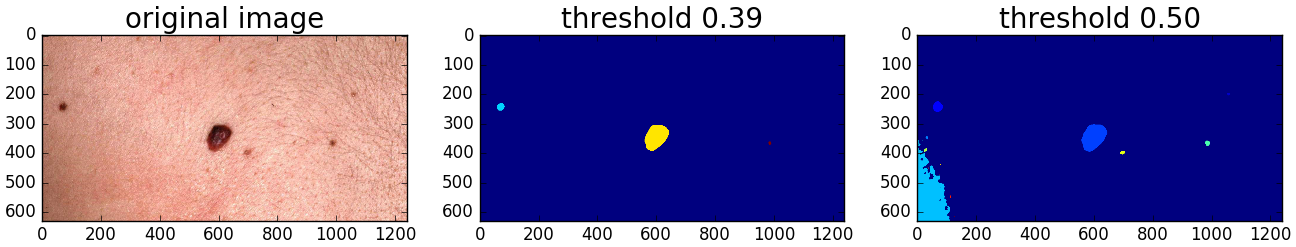
\includegraphics[width=\textwidth,keepaspectratio]{assets/image_processing/thresholding/figure_02.png}
    \caption{Threshold segmentation B}
    \label{fig:thresh_B}
\end{figure}
\begin{figure}[H]
    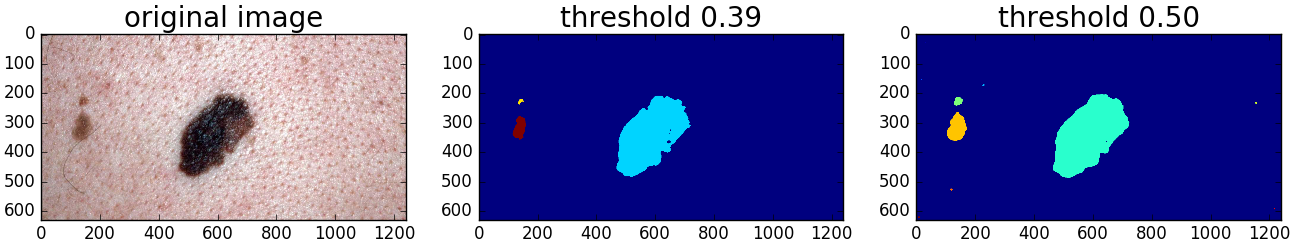
\includegraphics[width=\textwidth,keepaspectratio]{assets/image_processing/thresholding/figure_03.png}
    \caption{Threshold segmentation C}
    \label{fig:thresh_C}
\end{figure}
\begin{figure}[H]
    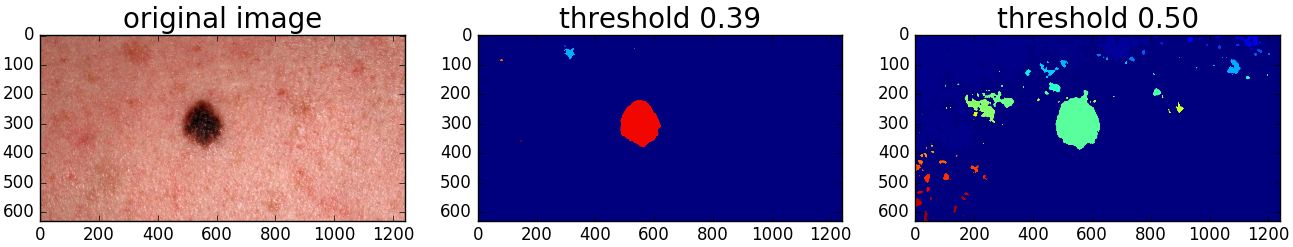
\includegraphics[width=\textwidth,keepaspectratio]{assets/image_processing/thresholding/figure_04.png}
    \caption{Threshold segmentation D}
    \label{fig:thresh_D}
\end{figure}

Depending on the content of the image and the threshold value used more regions are isolated than actually needed. It is fairly easy to discard the irrelevant regions based on some simple assumptions. We can assume that the most interesting region should be roughly in the center of the image, it should be larger than other regions, and it should not touch the edge of the image. The region remaining should be the main region of interest.

Other problems remain though. The regions of interest in figures \ref{fig:thresh_A} and \ref{fig:thresh_C} have some holes within the main region. Figure \ref{fig:thresh_D} has too much area selected at the higher threshold value, \ref{fig:thresh_A} has too little at the lower threshold setting. A static threshold setting will generally not achieve the same level of quality for all images.

By measuring the size of the main region of interest at different threshold values.

\subsection{Color Transformation and Analysis}

The thresholding method above only takes the brightness of the image into account, ignoring any colour variations. This seems counter intuitive though, especially considering the domain where one of the qualities of melanocytic nevi and melanoma is the high concentration of melanin which is responsible for skin pigmentation. It would seem natural that other image qualities such as hue and colour intensity would be important as well.

By transforming RGB images into HSV encoded image, other image qualities can be investigated more intuitively. HSV encoded images store colour information as hue ( colour spectrum ), saturation ( colour intensity ) and value ( brightness ).

By mapping the HSV values of an image into a 3d coordinate system where the coordinates are hue, saturation, and value some insights about the pixel grouping can be investigated. Figure \ref{fig:hsv_place} shows an image of a skin lesion next to the 3d transformation of the pixels in HSV Space. Hue and colour are the horizontal axes, value is the vertical axis.

Once can observe that the most of the pixels that make up the lesion area form a distinct clump that is connected to a larger clump that corresponds to the surrounding healthy skin.


\begin{figure}[H]
    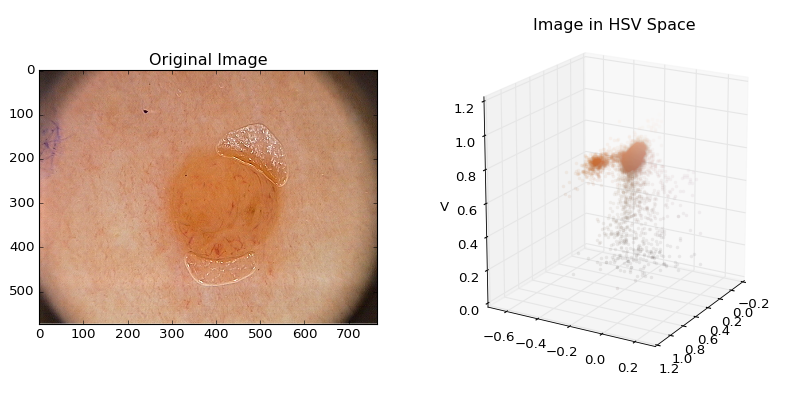
\includegraphics[width=\textwidth,keepaspectratio]{assets/image_processing/hsv/hsv_3dplot.png}
    \caption{HSV Space}
    \label{fig:hsv_place}
\end{figure}

In Figure \ref{fig:hsv_3d} the output of an application is displayed that highlights pixels in the original image that correspond to selected pixels in 3d HSV space.

\begin{figure}[H]
    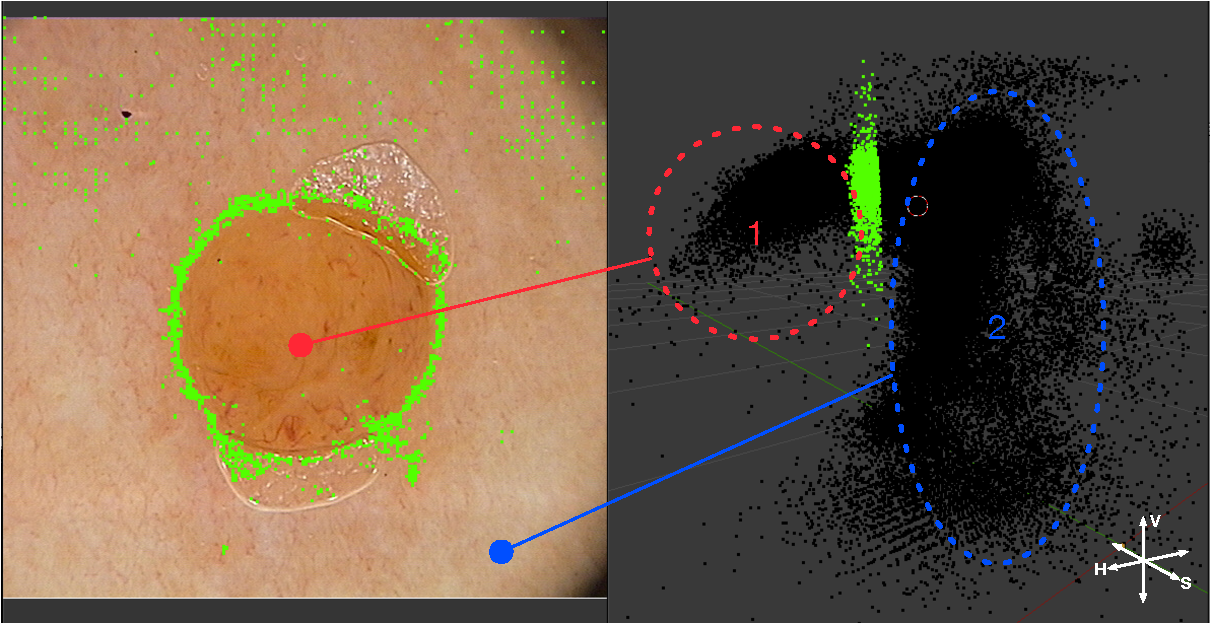
\includegraphics[width=\textwidth,keepaspectratio]{assets/image_processing/hsv/hsv_space.pdf}
    \caption{HSV Clustering visualization}
    \label{fig:hsv_3d}
\end{figure}

This application was implemented as a python script in the Blender 3d application. The script would allow an image to be loaded into memory. The pixels would be read pixel by pixel and a point corresponding to each pixel's HSV values would be positioned in a 3d coordinate system. Each point would hold a reference to it's corresponding pixel position in the original image.

Selecting the points in the 3d view would highlight the corresponding pixel in the original image. It is clearly visible that the points lying between the 2 main clusters (1 and 2 in Figure \ref{fig:hsv_3d}) correspond strongly with the pixels on the border between the skin lesion and the healthy surround skin area.

Some time was spent investigating methods of grouping pixels based on both their distance in HSV space and the distance in the image space but quickly put aside because of the time and effort considerations.

The research did lead to the discovery of an already available method called Simple Linear Iterative Clustering.

\subsection{SLIC Superpixels}

SLIC is a segementaion algorithm that produces Superpixels, large groups of pixels with similar content. The edges of the Superpixel shoudld correspond to edges of objects in an image.

The SLIC algorithm uses the 3 color and 2 dimensions to cluster pixels \cite{slic}. In an iterative and computationally efficient algorithm the image is first segmented into tiles. In each iteration the borders of the tiles are recalculated based on the similarity of the pixels in the surrounding area.

Figure \ref{fig:slic} illustrates the first 6 iterations of the SLIC algorithm on a skin lesion image.


\begin{figure}[H]
    \includegraphics[width=\textwidth,keepaspectratio]{assets/image_processing/slic/slic_01.png}
    \caption{SLIC superpixel segmentation}
    \label{fig:slic}
\end{figure}



